\documentclass{beamer}
\usetheme{Warsaw}

\usepackage[utf8]{inputenc}
\usepackage{default}
\usepackage{url}
\usepackage{tikz}
\usepackage{amsmath}
\usepackage{pst-node}
\usepackage{empheq}
\usetheme{Warsaw}
\useoutertheme{infolines}
\usepackage[absolute,overlay]{textpos}
\usetikzlibrary{matrix}
\setlength{\TPHorizModule}{\paperwidth}\setlength{\TPVertModule}{\paperheight}
\title{Co-occurrence statistics of the entities on the web}
\subtitle{Seminar Presentation}
\author[Aman Madaan]{Aman Madaan}
\institute[IITB]{
  Indian Institute of Technology Bombay, Mumbai
}
\date{May 2nd, 2014}
\addtobeamertemplate{navigation symbols}{}{%
    \usebeamerfont{footline}%
    \usebeamercolor[fg]{footline}%
    \hspace{1em}%
    \insertframenumber/\inserttotalframenumber
}

\newcommand*{\Comb}[2]{{}^{#1}C_{#2}}%

\usepackage{amsmath}
\usepackage{pst-node}

\usepackage{color}
\definecolor{myblue}{rgb}{.8, .8, 1}
\definecolor{mygreen}{rgb}{.8, 1, 0.8}



\newlength\mytemplen
\newsavebox\mytempbox

\makeatletter
\newcommand\mybluebox{%
    \@ifnextchar[%]
       {\@mybluebox}%
       {\@mybluebox[0pt]}}

\def\@mybluebox[#1]{%
    \@ifnextchar[%]
       {\@@mybluebox[#1]}%
       {\@@mybluebox[#1][0pt]}}

\def\@@mybluebox[#1][#2]#3{
    \sbox\mytempbox{#3}%
    \mytemplen\ht\mytempbox
    \advance\mytemplen #1\relax
    \ht\mytempbox\mytemplen
    \mytemplen\dp\mytempbox
    \advance\mytemplen #2\relax
    \dp\mytempbox\mytemplen
    \colorbox{myblue}{\hspace{1em}\usebox{\mytempbox}\hspace{1em}}}

\makeatother


\psset{arrowscale=2,arrows=->}
\def\VPh{\vphantom{\displaystyle\sum_{i=n}^m {i^2}}}
\def\psBox#1#2{\psframebox[fillcolor=#1,fillstyle=solid]{\VPh\displaystyle#2}}



\begin{document}
\maketitle
\begin{frame}{Motivation}


 \begin{itemize}
  \item Web Search is a quest for knowledge \medskip
  \item The open web is huge, \textbf{1.8 billion} indexed web pages\footnote{As of 31st March 2014}, but unstructured  \medskip
  \item The knowledge is scattered around in pieces \medskip
  \item A user needs to carve the structure out of the web  \medskip
  \item Structuring the web : A web page is more than just a bundle of strings \medskip
  \item Benefits are not limited to search! \medskip
 \end{itemize}

\end{frame}


\begin{frame}{Structuring the web}
 \begin{itemize}
  \item Learn what the text is all about \medskip
  \item Go beyond Strings \medskip
  \item ``Albert Einstein'' \medskip
  \item Beyond the tricks like finding pages having the \textbf{String} ``Albert Einstein'', \medskip
  pages which link to pages having the \textbf{String} ``Albert Einstein''
 \end{itemize}

\end{frame}

\begin{frame}
\begin{exampleblock}{}
  {\large ``Words that you use when you are doing the search, well they aren't \emph{just words}, they refer to \textbf{real} things
in the world``}
  \vskip5mm
  \hspace*\fill{\small--- Jack Menzel, Product Management Director, Google Knowledge Graph
}
\end{exampleblock}
\end{frame}

\begin{frame}
 \frametitle{Words are not just words}
\begin{textblock*}{100pt}[.50,.5](190pt,170pt)
\begin{figure}[h]
 \centering
 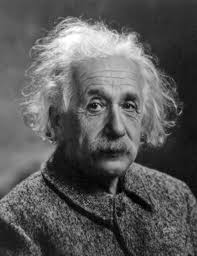
\includegraphics[bb=0 0 197 256,scale=0.5]{./einstein.jpg}
  \caption{Albert Einstein}
 % einstein.jpg: 197x256 pixel, 72dpi, 6.95x9.03 cm, bb=0 0 197 256
\end{figure}
\end{textblock*}
\end{frame}
\begin{frame}
 \frametitle{Words are not just words}
\begin{textblock*}{100pt}[.50,.5](190pt,170pt)
\begin{figure}[h]
 \centering
 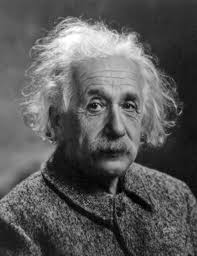
\includegraphics[bb=0 0 197 256,scale=0.5]{./einstein.jpg}
  \caption{Albert Einstein}
 % einstein.jpg: 197x256 pixel, 72dpi, 6.95x9.03 cm, bb=0 0 197 256
\end{figure}
\end{textblock*}
\begin{textblock*}{80pt}[.50,.5](60pt,70pt)
\begin{figure}[h]
 \centering
 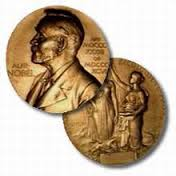
\includegraphics[bb=0 0 197 256,scale=0.5]{./nobel.jpg}
 % einstein.jpg: 197x256 pixel, 72dpi, 6.95x9.03 cm, bb=0 0 197 256
\end{figure}
\end{textblock*}

\end{frame}
\begin{frame}
 \frametitle{Words are not just words}
\begin{textblock*}{100pt}[.50,.5](190pt,170pt)
\begin{figure}[h]
 \centering
 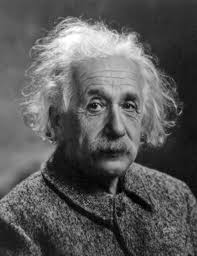
\includegraphics[bb=0 0 197 256,scale=0.5]{./einstein.jpg}
  \caption{Albert Einstein}
 % einstein.jpg: 197x256 pixel, 72dpi, 6.95x9.03 cm, bb=0 0 197 256
\end{figure}
\end{textblock*}
\begin{textblock*}{80pt}[.50,.5](60pt,70pt)
\begin{figure}[h]
 \centering
 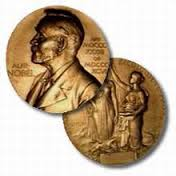
\includegraphics[bb=0 0 197 256,scale=0.5]{./nobel.jpg}
 % einstein.jpg: 197x256 pixel, 72dpi, 6.95x9.03 cm, bb=0 0 197 256
\end{figure}
\end{textblock*}

\begin{textblock*}{80pt}[.50,.5](60pt,170pt)
\begin{figure}[h]
 \centering
 
\includegraphics[bb=0 0 197 256,scale=0.5]{./zurich.jpg}
 % einstein.jpg: 197x256 pixel, 72dpi, 6.95x9.03 cm, bb=0 0 197 256
\end{figure}
\end{textblock*}

\end{frame}
\begin{frame}
 \frametitle{Words are not just words}
\begin{textblock*}{100pt}[.50,.5](190pt,170pt)
\begin{figure}[h]
 \centering
 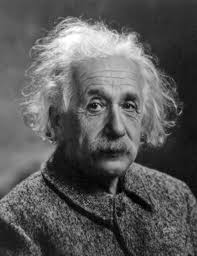
\includegraphics[bb=0 0 197 256,scale=0.5]{./einstein.jpg}
 % einstein.jpg: 197x256 pixel, 72dpi, 6.95x9.03 cm, bb=0 0 197 256
 \caption{Albert Einstein}
\end{figure}
\end{textblock*}
\begin{textblock*}{80pt}[.50,.5](60pt,70pt)
\begin{figure}[h]
 \centering
 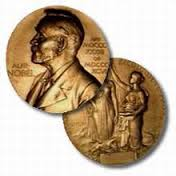
\includegraphics[bb=0 0 197 256,scale=0.5]{./nobel.jpg}
 % einstein.jpg: 197x256 pixel, 72dpi, 6.95x9.03 cm, bb=0 0 197 256
\end{figure}
\end{textblock*}

\begin{textblock*}{80pt}[.50,.5](60pt,170pt)
\begin{figure}[h]
 \centering
 
\includegraphics[bb=0 0 197 256,scale=0.5]{./zurich.jpg}
 % einstein.jpg: 197x256 pixel, 72dpi, 6.95x9.03 cm, bb=0 0 197 256
\end{figure}
\end{textblock*}


\begin{textblock*}{120pt}[.50,.5](310pt,70pt)
\begin{itemize} 
\item \textbf{Born :} 1879, Germany
\item \textbf{Died :} 1955, US
 \end{itemize}
\end{textblock*}
\end{frame}
\begin{frame}
 \frametitle{Words are not just words}
\begin{textblock*}{100pt}[.50,.5](190pt,170pt)
\begin{figure}[h]
 \centering
 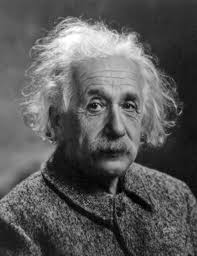
\includegraphics[bb=0 0 197 256,scale=0.5]{./einstein.jpg}
 % einstein.jpg: 197x256 pixel, 72dpi, 6.95x9.03 cm, bb=0 0 197 256
 \caption{Albert Einstein}
\end{figure}
\end{textblock*}
\begin{textblock*}{80pt}[.50,.5](60pt,70pt)
\begin{figure}[h]
 \centering
 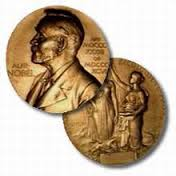
\includegraphics[bb=0 0 197 256,scale=0.5]{./nobel.jpg}
 % einstein.jpg: 197x256 pixel, 72dpi, 6.95x9.03 cm, bb=0 0 197 256
\end{figure}
\end{textblock*}

\begin{textblock*}{80pt}[.50,.5](60pt,170pt)
\begin{figure}[h]
 \centering
 
\includegraphics[bb=0 0 197 256,scale=0.5]{./zurich.jpg}
 % einstein.jpg: 197x256 pixel, 72dpi, 6.95x9.03 cm, bb=0 0 197 256
\end{figure}
\end{textblock*}


\begin{textblock*}{120pt}[.50,.5](310pt,70pt)
\begin{itemize} 
\item \textbf{Born :} 1879, Germany
\item \textbf{Died :} 1955, US
 \end{itemize}

\end{textblock*}

\begin{textblock*}{120pt}[.50,.5](310pt,170pt)
''Entities'' \emph{like} Albert Einstein
\begin{itemize} 
\item \textbf{Born :} Issac Newton
\item \textbf{Died :} Stephen Hawking
 \end{itemize}
\end{textblock*}

\end{frame}


\begin{frame}{Structuring the web : Knowledge Bases}
\begin{itemize}
 \item Need a standard reference set of entities
 \item Wordnet : The maiden knowledge base, has clean type system but limited entity base
 \item Development of Wikipedia has lead to the development of large knowledge bases
\end{itemize}
\end{frame}

\begin{frame}{Freebase}
\begin{figure}[h]
 \centering
 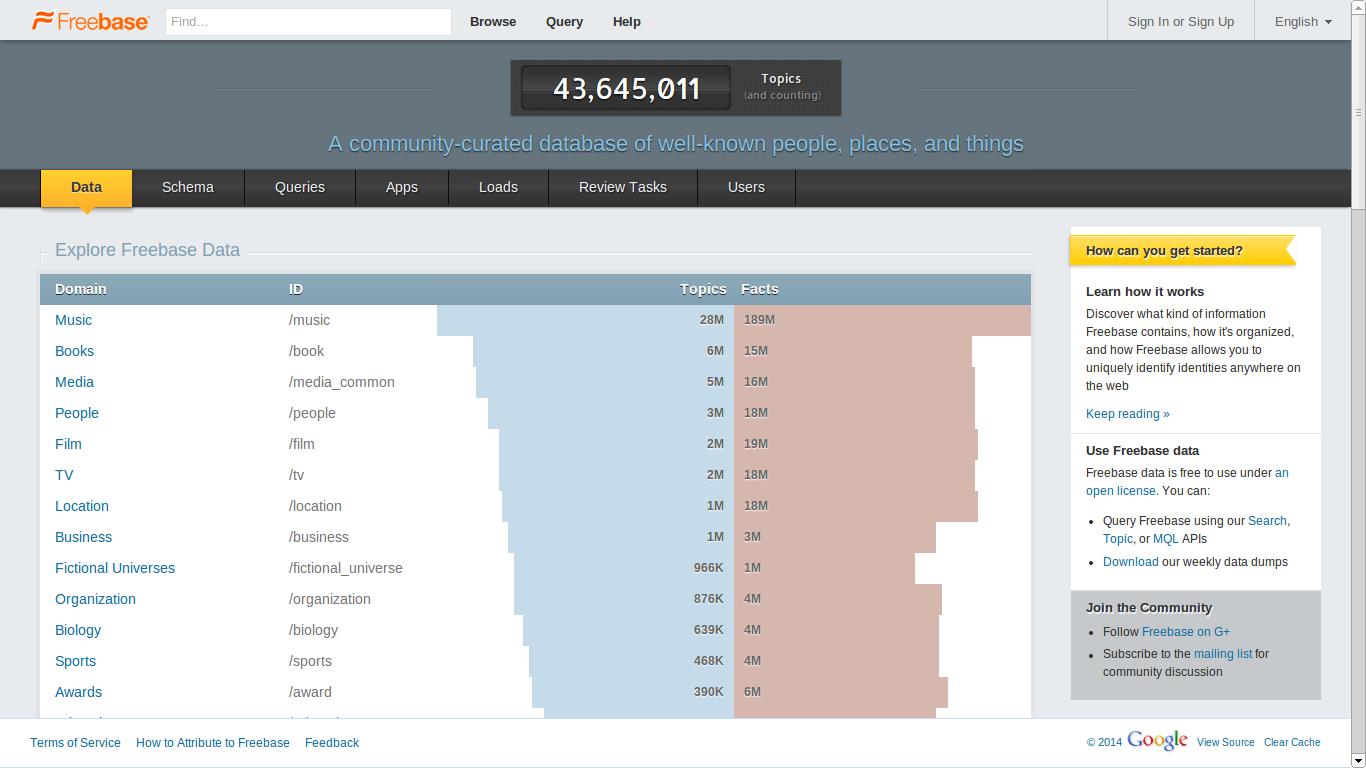
\includegraphics[bb=0 0 1366 768,scale=0.25]{./freebase.png}
 % freebase.png: 1366x768 pixel, 72dpi, 48.19x27.09 cm, bb=0 0 1366 768
\end{figure}
 
\end{frame}
\begin{frame}{Freebase}
\begin{itemize}
 \item Freebase relies on crowd sourcing for creation of a rich but clean knowledge base \medskip
 \item The development of Freebase follows the same chain as Every local disambiguation techniques fall into one
Wikipedia, with users flagging issues, and cleaning and augmenting information \medskip
\item Freebase also provides access to itself using web APIs.
\end{itemize}
\end{frame}

\begin{frame}{Knowledge Bases : Not there yet}
 \begin{itemize}
  \item None of the knowledge bases to the best of my knowledge provides any kind of entity priors
  of any kind
  \item These pieces of information are really crucial for a number of tasks related to querying knowledge
  graphs.
  \begin{alertblock}{Alert-block title}
This is a block in red
\end{alertblock}
  \item We motivate the need for such statistics after reviewing named entity disambiguation techniques. 
 \end{itemize}

\end{frame}


\begin{frame}{Aggregate Statistics}
\begin{itemize}
\item So the Internet is made up of things, the entities, which have dependencies and affiliations with other entities  \medskip
\item It makes sense to ask which of these “things” are more important than the others. \medskip
\item We need just the statistics about occurrence of the entities. \medskip
\item Which of the entities appear together often? \medskip
\item Which of the entities appear in pair often? In triples? \medskip	
\item Named Entity Disambiguation
\end{itemize}
\end{frame}


\begin{frame}

 \begin{center}
 \usebeamerfont*{frametitle}
 \Huge  \color{blue}{Named Entity Disambiguation}
  
  \bigskip

  \end{center}

\end{frame}

\begin{frame}{One Thousand Words}
 \begin{figure}[h]
 \centering
 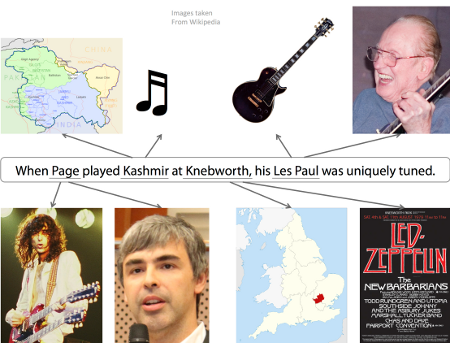
\includegraphics[bb=0 0 216 165]{./ned.png}
 % ned.png: 450x343 pixel, 150dpi, 7.62x5.81 cm, bb=0 0 216 165
 \caption{The Problem Of Named Entity Disambiguation}
\end{figure}

\end{frame}


\begin{frame}
 \frametitle{Recognition and Tagging : Two step problem}
 \begin{center}
\textcolor{blue}{Michael Jordan is a Professor at Berkeley}
   \end{center}

\end{frame}

\begin{frame}
 \frametitle{Recognition and Tagging : Two step problem}
 \begin{center}
\textcolor{blue}{Michael Jordan is a Professor at Berkeley}
   \end{center}

 \begin{itemize}  
  \item Step 1 : \textbf{Identify} entities

  \medskip
  \textcolor{green}{Michael Jordan\_PERSON} is a professor at \textcolor{green}{Berkeley\_INSTITUTION} \medskip
  
\end{itemize}
\end{frame}

\begin{frame}
 \frametitle{Recognition and tagging : Two step problem}
 \begin{center}
\textcolor{blue}{Michael Jordan is a Professor at Berkeley}
   \end{center}

 \begin{itemize}  
  \item Step 1 : \textbf{Identify} entities
  \medskip
  
  \textcolor{green}{Michael Jordan\_PERSON} is a professor at \textcolor{green}{Berkeley\_INSTITUTION} \medskip
  \item Step 2 : \textbf{Link} entities to knowledge bases : 
  \medskip
  
  \textcolor{red}{Michael Jordan\_ENTITY} (\url{http://en.wikipedia.org/wiki/Michael_I._Jordan})  is a professor at  
  \textcolor{red}{Berkeley\_ENTITY} (\url{http://en.wikipedia.org/wiki/University_of_California,_Berkeley})
\end{itemize}

\end{frame}

\begin{frame}
\frametitle{NER : Problem Statement}
 \begin{center}
\  \begin{definition}[Named entity recognition\footnote {from \ref{thewiki}}]
   Named-entity recognition (NER) (also known as entity identification and entity extraction) is a subtask of information extraction that seeks to locate and classify 
   atomic elements in text into predefined categories such as the names of persons, organizations, locations, expressions of times, quantities, monetary values, percentages, etc.
  \end{definition}

 \end{center}
\end{frame}

\begin{frame}
 \frametitle{NER : Solutions}
 \begin{center}
 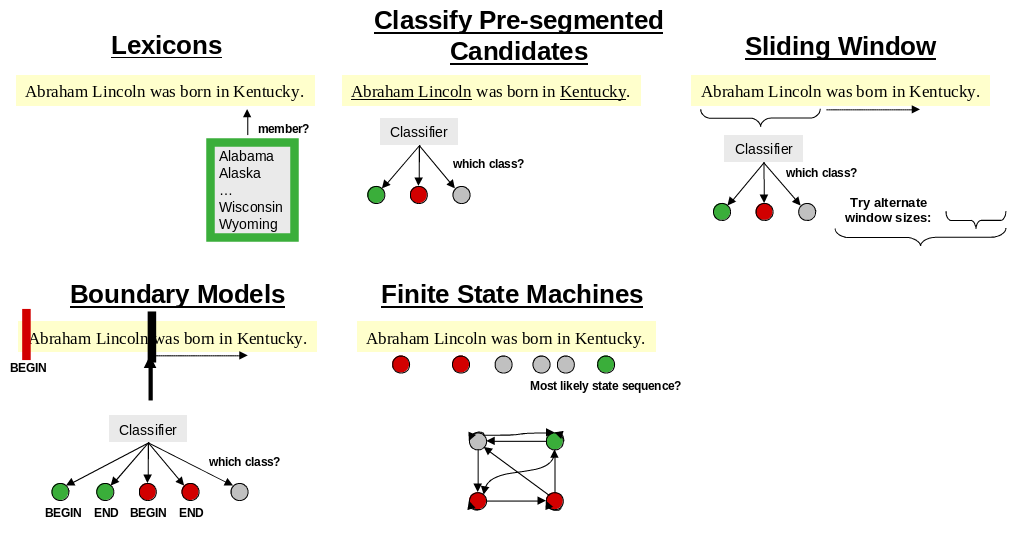
\includegraphics[height = 6cm]{cohen}\footnote{from \ref{thesurvey}}
 \end{center}

\end{frame}

 \begin{frame}
 \frametitle{NER as a sequence labeling problem}
 \begin{itemize}
  \item Observation sequence : Text \medskip
  \item State sequence : Labeling of the sequence with elements in (PER, LOC, ORG) etc. \medskip
  \item Find $\text{argmax}_{S}  P(S|O)$ \medskip
  \item Candidates : HMM, MEMM, CRF
  \end{itemize}
\end{frame}

\begin{frame}
 \frametitle{NER as a sequence labeling problem}
 \begin{itemize}
 \item \textbf{HMM} 
 \begin{itemize}
 \item Generative
 \item Makes strong independence assumption
 \item Myopic (Refer to label bias problem in \hyperref[thesurvey]{William Cohen's Survey})
 \end{itemize}
 
 \item \textbf{MEMM}
 \begin{itemize}
 \item Discriminative
 \item No independence assumptions are made, by formulation
 \item Allows the use of feature functions
 \item Myopic
 \end{itemize}
 
 \item \textbf{CRF}
 \begin{itemize}
  \item Discriminative
  \item MEMM + non myopic, avoids local normalization
  \item Talks of ``compatibility'', not independence (\hyperref[thesite]{CS 728})
 \end{itemize}

 
 \end{itemize}
 
\end{frame}
\begin{frame}{Named Entity Disambiguation : Outline}


 \begin{itemize}
  \item Techniques
  \begin{itemize}
   \item Local Disambiguation \medskip
   \item Collective Disambiguation \medskip
   \item Robust Disambiguation of Named Entities \medskip
  \end{itemize}
  \item Quick Demo
 \end{itemize}

\end{frame}
\begin{frame}{Local Disambiguation}
 \begin{itemize}
  \item Resolve each mention oblivious to the other disambiguations \medskip
  \item Need to disambiguate a mention by collecting the local evidences \medskip
  \item \textbf{Evidences}  POS tags, gender information, dictionary lookup \medskip
  \item \textbf{Local}  We cannot use the disambiguation information for any of the other entities for solving the problem \medskip
  \item Techniques
  \begin{itemize} 
  \item Machine Learning Based
  \item Rule Based
  \item Recent Rule based 
 \end{itemize}
 \end{itemize}
 

\end{frame}
\begin{frame}{Local Disambiguation : Rule Based}
\begin{itemize}
 \item Stems from the classical problem of word sense disambiguation \medskip
 \item Example : Lesk's Algorithm \medskip
  \begin{block}{Lesk's Algorithm} \medskip
       
 For each mention, pick the candidate sense for which there is maximum overlap
 in the gloss (definition) of the candidate and the context
\end{block}
\item Note that the possible mentions are those that are identified by the named entity recognizer
 \end{itemize}

 
\end{frame}


\begin{frame}{Local Disambiguation : Rule Based (Example)}
\begin{itemize}
\item Consider the same example
 \begin{figure}[h]
 \centering
 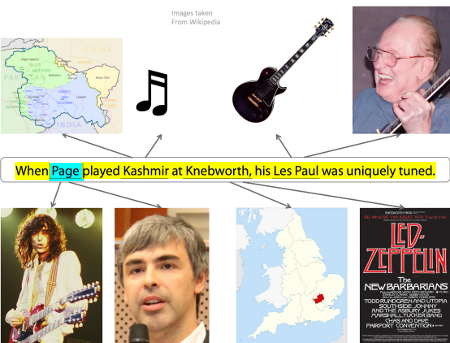
\includegraphics[bb=0 0 216 165]{./nedrulebased.png}
 % ned.png: 450x343 pixel, 150dpi, 7.62x5.81 cm, bb=0 0 216 165
 \caption{Disambiguating ``Page``}
\end{figure}
\item Disambiguating ``Page''
\end{itemize}
\end{frame}
\begin{frame}{Local Disambiguation : Rule Based (Example)}
 \begin{itemize}
  \item \textbf{Jimmy Page}\footnote{First para of the Wikipedia Entry} James Patrick "Jimmy" Page, OBE (born 9 January 1944) is an English musician, songwriter and record producer who achieved international success as the \textcolor{red}{guitar player} and leader of the rock band Led Zeppelin.
  \item \textbf{Larry Page}\footnote{First para of the Wikipedia Entry}	 Lawrence "Larry" Page[2] (born March 26, 1973) is an American Business magnate and computer scientist who is the co-founder of Google, alongside Sergey Brin. On April 4, 2011, Page succeeded Eric Schmidt as the chief executive officer of Google.[3][4] As of 2014, Page's personal wealth is estimated to be US\$32.3 billion, ranking him \#19 on the Forbes list of billionaires.[1]
  \item \textbf{Context} \textcolor{red}{played} kashmir at Knebworth, his Les paul was uniquely tuned
  
 \end{itemize}
\textcolor{green}{\textbf{\emph{Pick the candidate that is most likely given the context}}}
\end{frame}
\begin{frame}{Local Disambiguation : Rule based : Drawbacks}
\begin{itemize}
 \item Context can be misleading \bigskip
 \textcolor{green}{\emph{Amazon} saw a flood of visitors} \bigskip
 \item Context can be insufficient (or even absent!)
 
\end{itemize}

 
\end{frame}


\begin{frame}{Collecting Statistics of interest I : Sense Prior}
\begin{itemize}

\item \textbf{Sense Prior} The number of times a particular ``sense'' of an entity is used \medskip
\item There are several ``Gingerbreads'' (Android 2.3, The novel) \medskip
\item Sense prior would tell us how frequent is \emph{Gingerbread the OS} compared with \emph{Gingerbread the novel}  \medskip
\item $Sense Prior(Si , E) = P (\text{E appears as the ith sense}) = P (Si |E) $ \medskip
\item Different from mention prior! (Number of times a mention links to a particular entity)
\end{itemize}
\end{frame}

\begin{frame}{Sense Prior : Example (Hypothetical)}
  \begin{textblock*}{120pt}[.50,.5](70pt,70pt)
  \begin{figure}[h]
 
 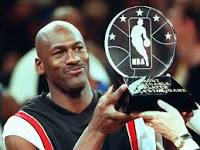
\includegraphics[bb=0 0 200 150, scale=0.4]{./baske.jpg}
 
 % baske.jpg: 200x150 pixel, 72dpi, 7.06x5.29 cm, bb=0 0 200 150
\end{figure}
   \centering 
   Basketballer (60\%)
\end{textblock*}
  \begin{textblock*}{120pt}[.50,.5](280pt,80pt)
  \begin{figure}[h]
 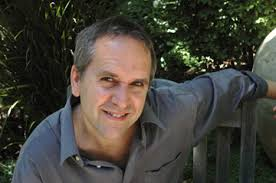
\includegraphics[bb=0 0 200 150, scale=0.4]{./prof.jpg}
 % baske.jpg: 200x150 pixel, 72dpi, 7.06x5.29 cm, bb=0 0 200 150
\end{figure}
\centering
   Professor (30\%)
\end{textblock*}
  \begin{textblock*}{120pt}[.50,.5](70pt,200pt)
  \begin{figure}[h]
 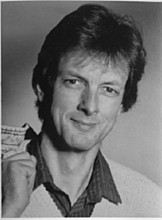
\includegraphics[bb=0 0 200 150, scale=0.4]{./botanist.jpg}
 % baske.jpg: 200x150 pixel, 72dpi, 7.06x5.29 cm, bb=0 0 200 150
\end{figure}
\centering
Botanist (8\%)
\end{textblock*}
  \begin{textblock*}{120pt}[.50,.5](260pt,200pt)
  \begin{figure}[h]
 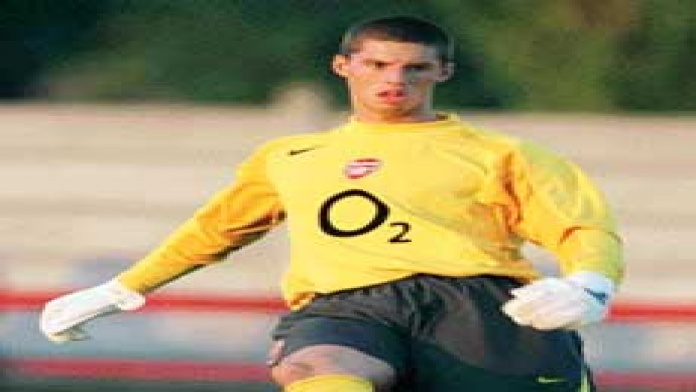
\includegraphics[bb=0 0 200 150, scale=0.16]{./footballer.jpg}
 % baske.jpg: 200x150 pixel, 72dpi, 7.06x5.29 cm, bb=0 0 200 150
\end{figure}
\centering
Footballer (2\%)
\end{textblock*}
  \begin{textblock*}{120pt}[.50,.5](200pt,140pt)

\large{Michael Jordan}

\end{textblock*}

\end{frame}

\begin{frame}{Co occurrence statistics}
\begin{itemize}
 \item \textbf{Entity Bigrams} Counts the number of times two given entities, taking two given senses appear together. \medskip
\item Eg. : Number of times Nokia \url{http://en.wikipedia.org/wiki/Nokia} appears with Gingerbread \url{http://en.wikipedia.org/wiki/Gingerbread_(operating_system)} \medskip


 \item $\text{Entity Bi Gram}(E2|E1) = P (E2\ follows\ E1) = P (E2|E1)$
 \end{itemize}
\end{frame}

\begin{frame}{Co occurrence statistics : Example}
 \begin{figure}[h]
 \centering
 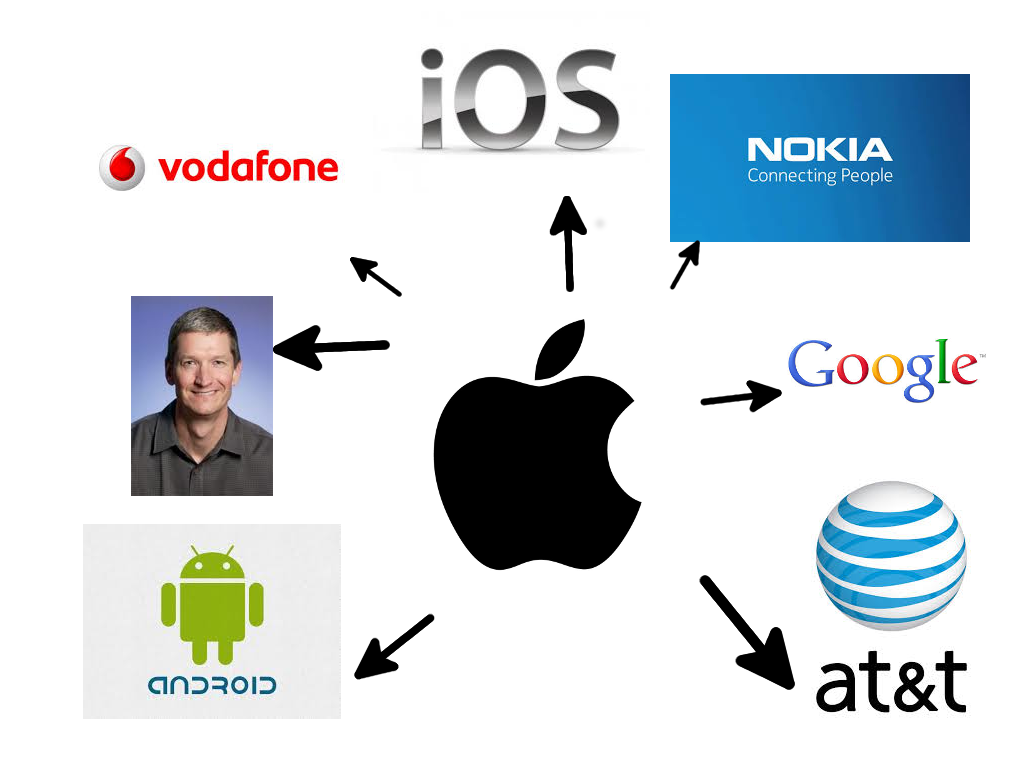
\includegraphics[bb=0 0 1024 768, scale=0.25]{./entitycoocc.png}
 % entitycoocc.png: 1024x768 pixel, 72dpi, 36.12x27.09 cm, bb=0 0 1024 768
 \caption{Entities Frequently Appear with related entities}
\end{figure}

\end{frame}




\begin{frame}
\begin{center}
 
  Collective Annotation of WikiPedia Entities in Web Text 
  
  \bigskip
  
 \hyperref[thepaper]{ Sayali Kulkarni, Amit Singh, Ganesh Ramakrishnan, and Soumen Chakrabarti}
  \end{center}

\end{frame}

\begin{frame}
 \frametitle{Key Intuition : Topical Coherence}
 \begin{itemize}
  \item A document is usually about one topic \bigskip
  \item Disambiguating each entity using the local clues misses out on a major piece of information : Topic of a page \bigskip
  \item A page is usually has one topic, you can expect all the entities to be \emph{related} to the topic \emph{somehow} \bigskip
  \end{itemize}
  \textcolor{green}{Michael Jackson} : 30 Disambiguations 
  
 \textcolor{green}{John Paul} : 10 disambiguations 
 
 
 
  But if they are mentioned on the \textbf{same page}, the page is most likely about Christianity, A big hint towards disambiguating \textbf{both} of them
  
 
  \end{frame}
\begin{frame}{Topical Coherence}
  \begin{figure}[h]
 \centering
 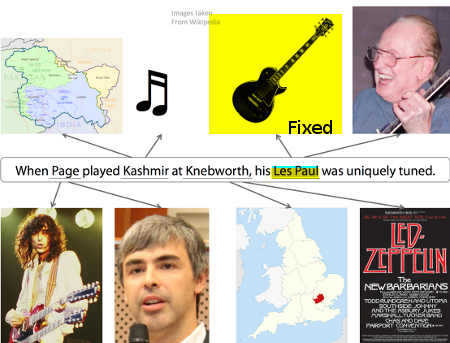
\includegraphics[bb=0 0 216 165]{./nedcollective.png}
 % nedcollective.png: 450x343 pixel, 150dpi, 7.62x5.81 cm, bb=0 0 216 165
\end{figure}

 \end{frame}

\begin{frame}{Challenges}
 \begin{itemize}
  \item Capturing local compatibility \medskip
  \begin{itemize}
   \item \textcolor{blue}{Create a scoring function to rank possible candidates}
  \end{itemize}

  \item Inculcating topical coherence in the overall objective \medskip

  \begin{itemize}
   \item \textcolor{blue}{Define Topical coherence}
  \end{itemize}

  \end{itemize}

\end{frame}

\begin{frame}
 \frametitle{Local compatibility}
 \begin{itemize}
  \item $s$ : Spot, an Entity to be disambiguated (Christian leader John Paul) \bigskip 
  \item $\gamma$ : An entity label value (\url{http://en.wikipedia.org/wiki/Po-pe_John_Paul_II})  \bigskip 
 \item $f_s(\gamma)$ : A feature function that creates a vector of features
 \end{itemize}

  
\end{frame}

\begin{frame}

\frametitle{Local compatibility : Feature design} 
\begin{itemize}
 \item 1. Take
\begin{itemize} 
 \item Text from the first descriptive paragraph of $\gamma$
  \item Text from the whole page for $\gamma$
  \item Anchor text within Wikipedia for $\gamma$.
  \item Anchor text and 5 tokens around $\gamma$ 
 \end{itemize}
 
 \item 2. Apply each of the following operation with one argument as Spot
    \begin{itemize}
      \item{Dot-product between word count vectors}
      \item{Cosine similarity in TFIDF vector space}
      \item{Jaccard similarity between word sets}
 \end{itemize} 
 \end{itemize}
 Total 12 Features (3 operations, 4 argument pairs) + Sense Probability Prior\footnote{Obtained by counting intra wiki links}
 
\end{frame}

\begin{frame}
 \frametitle{Compatibility Score}
 \begin{itemize}
 \item Local compatibility score between a spot $s$ and a candidate is given by $w^{T}f_s(\gamma)$ \medskip
 \item Thus, candidate is picked by $argmax_{\gamma\in\Gamma}w^{T}f_s(\gamma)$ \medskip
 \item $w$ is trained using an SVM like training objective 
 
 \begin{center} 
 Minimize $||w||^2 + C\Sigma_{s}\varepsilon_s$
 under the constraints
 $w^{T}f_s(\gamma) - w^{T}f_s(\gamma) \geq 1 - \varepsilon_s$ \end{center}
 \end{itemize}
 
 \end{frame}

\begin{frame}{Defining topic Relatedness}
  \begin{itemize}
   \item We need some notion of capturing the fact that 2 topics are related to each other \medskip
   \item Given
   \begin{itemize}
    \item $g(\gamma)$ : Set of wikipedia pages that link to $\gamma$
    \item $c :$ Total number of Wikipedia pages
    \item $r(\gamma, \gamma') :$ Relatedness of topics $\gamma$ and $\gamma'$
   \end{itemize}\bigskip

    
   \item Define $ r(\gamma, \gamma') = \frac{log|g(\gamma) \bigcap g(\gamma')| - log(max\{|g(\gamma)|, |(\gamma')|\})} {log c - log(min\{|g(\gamma)|, |(\gamma')|\})}$ 
  (The Milne and Witten Score)
  \end{itemize}

  
 \end{frame}

 
\begin{frame}
  \frametitle{The Dominant Topic Model}
  \begin{itemize}
   \item Need to define a collective score based on pairwise topical coherence of all $\gamma_s$ used for labeling. \medskip
   \item The pairwise topical coherence, $r(\gamma_s, \gamma_s')$ is as defined above.\medskip
   \item For a page, overall topical coherence : \begin{center}\medskip
                                                  $\Sigma_{s \neq s' \in S_0}r(\gamma_s, \gamma_s')$
                                                 \end{center}
   \item Can be written as clique potential as in case of node potential\medskip
      \begin{center}
	$exp(\Sigma_{s \neq s' \in S_0}r(\gamma_s, \gamma_s'))$
      \end{center}

  \end{itemize}

 \end{frame}

\begin{frame}
  \frametitle{The Optimization objective}
 \begin{center}
 \begin{empheq}[box={\mybluebox[5pt]}]{equation*}
  \frac{1}{\binom{|S_0|}{2}}\Sigma_{s \neq s' \in S_0}r(\gamma_s, \gamma_s') + \frac{1}{|S_0|}\Sigma_{s \in S_0}w^{T}f_s(\gamma)
 \end{empheq}
 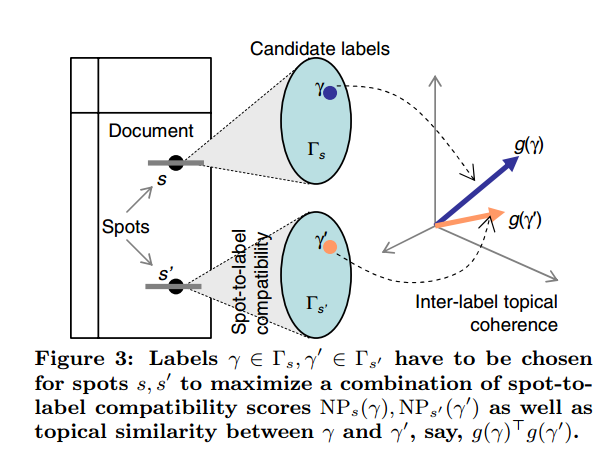
\includegraphics[height = 5 cm]{objective}\footnote{From \ref{thepaper}}
  \end{center}

 
 \end{frame}

\begin{frame}
  \frametitle{Solving the optimization objective}
  \begin{itemize}
   \item LP rounding approach\bigskip
   \item Hill climbing
   \begin{center}
    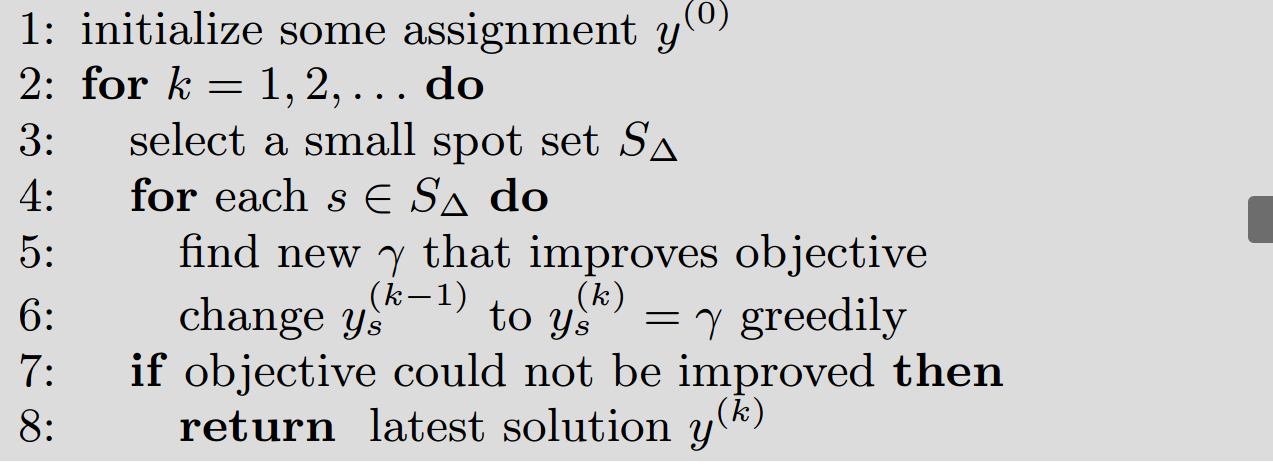
\includegraphics[height = 3cm]{hill}
   \end{center}

  \end{itemize}

 \end{frame}

\begin{frame}
  \frametitle{Experiments : Data preparation}
  \begin {itemize}
  \item August 2008 version of WikiPedia used, 5.15 million entity IDs. \medskip
  \item Filter out IDs composed of verbs, adverbs, conjunctions etc. \medskip
  \item Create a trie from IDs. \medskip
  \item Identify spots (\emph{NER}) by tokenizing the document and then matching spots with the trie. 
  \end{itemize}
  
 \end{frame}

\begin{frame}
  \frametitle{Experiments : Preparing Ground Truth Collection}
  \begin {itemize}
  \item Need data annotated with links to Wikipedia \medskip
  \item Done manually, pages obtained from popular links across various domains \medskip
  \item 19, 000 annotations marked, 40\% marked NA, 3800 distinct entities used \medskip
  \end{itemize}
 \begin{tabular}{| l | c | r |}
\hline
 Number of documents & 107 \\
Total number of spots & 17,200 \\

Spot per 100 tokens & 30 \\
Average ambiguity per Spot & 5.3\\
\hline
\end{tabular}
  
 \end{frame}

\begin{frame}
  \frametitle{Results : Only Local disambiguation}
  \begin{itemize}
  \item Local approach performs well
  \end{itemize}
  
  \begin{center}
  \begin{empheq}[box={\mybluebox[5pt]}]{equation*}
  \gamma_0 \leftarrow argmax_{\gamma\in\Gamma_s}  w^{T}f_s(\gamma)
  \end{empheq}
  \begin{empheq}[box={\mybluebox[5pt]}]{equation*}
  \text{if }  w^{T}f_s(\gamma_0) > \rho_{NA} \text{ then return }\gamma_0 \text{ else return NA}
  \end{empheq}
  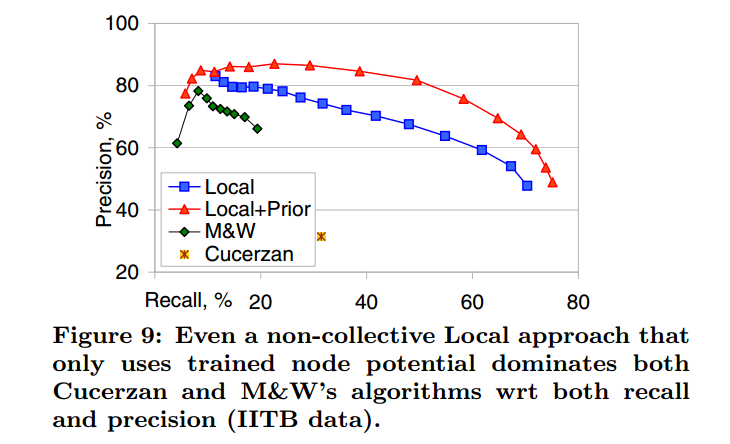
\includegraphics[height = 4 cm]{localperf}\footnote{from \ref{thepaper}}
  \end{center}

 \end{frame}

\begin{frame}
  \frametitle{LP vs Hill climbing approach}
  \begin{itemize}
   \item Hill climbing and LP are equivalent
  \end{itemize}

  \begin{center}
  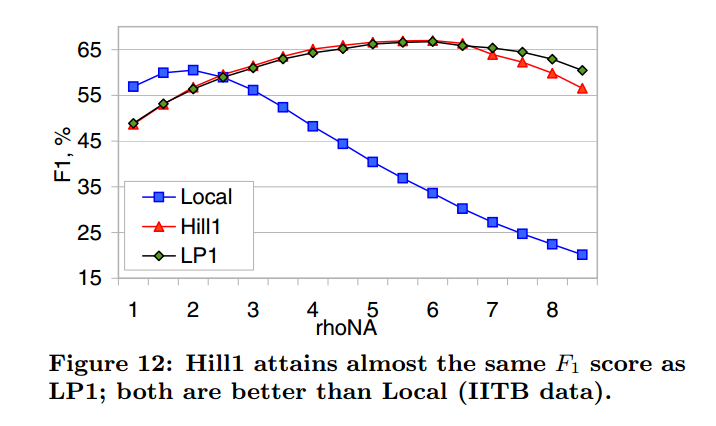
\includegraphics[height = 5 cm]{hillversuslp}\footnote{from \ref{thepaper}}
  \end{center}
 \end{frame}

 
\begin{frame}
  \frametitle{Recall precision for various approaches}
  \begin{itemize}
   \item Exploiting topical coherence improves precision by 9%
   \item Adding topic prior also helps
  \end{itemize}

  \begin{center}
  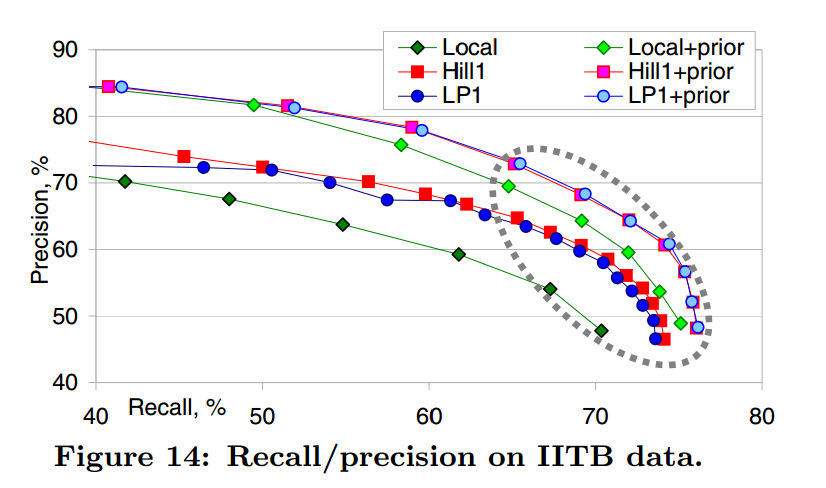
\includegraphics[height = 5 cm]{overall}\footnote{from \ref{thepaper}}
  \end{center}
 \end{frame}

\begin{frame}[allowframebreaks]
\frametitle{References}
\setbeamertemplate{bibliography item}[text]
\begin{thebibliography}{9}

\bibitem{A} \label{thepaper} Kulkarni, Sayali, et al. ``Collective annotation of Wikipedia entities in web text.'' Proceedings of the 15th ACM SIGKDD international conference on Knowledge discovery and data mining. ACM, 2009.

\bibitem{B}  \label{thesite} \url{http://www.cse.iitb.ac.in/~soumen/OWI/Slides/}

\bibitem{C} \label{thesurvey} William Cohen's Survey available at \ref{thesite}

\bibitem{The Wikipedia Page} \label{thewiki} \url{http://en.wikipedia.org/wiki/Named-entity_recognition}
\bibitem{D} \label{stanfordner} \url{http://nlp.stanford.edu/software/CRF-NER.shtml}

\bibitem{E} 

\label{mw}
Milne, David, and Ian H. Witten. ``Learning to link with wikipedia.'' Proceedings of the 17th ACM conference on Information and knowledge management. ACM, 2008.

\bibitem{F}{ws} \label{ws} \url{http://www.worldwidewebsize.com/}

\bibitem{G} \label{wikistats} \url{http://en.wikipedia.org/wiki/Wikipedia:Statistics}

\bibitem{F} \label{wikify}
Mihalcea, Rada, and Andras Csomai. ``Wikify!: linking documents to encyclopedic knowledge.'' Proceedings of the sixteenth ACM conference on Conference on information and knowledge management. ACM, 2007.

\bibitem{H} \label{aida}
Hoffart, Johannes, et al. ``Robust disambiguation of named entities in text.'' Proceedings of the Conference on Empirical Methods in Natural Language Processing. Association for Computational Linguistics, 2011.

\bibitem{I} \label{kpsim}
Hoffart, Johannes, et al. "Kore: keyphrase overlap relatedness for entity disambiguation." Proceedings of the 21st ACM international conference on Information and knowledge management. ACM, 2012.

\bibitem{J} \label{relgram}
Balasubramanian, Niranjan, Stephen Soderland, and Oren Etzioni. "Rel-grams: a probabilistic model of relations in text." Proceedings of the Joint Workshop on Automatic Knowledge Base Construction and Web-scale Knowledge Extraction. Association for Computational Linguistics, 2012.

\bibitem{H} \label{cohschemas}
Balasubramanian, Niranjan, Stephen Soderland, and Oren Etzioni Mausam. "Generating Coherent Event Schemas at Scale." Proceedings of the Empirical Methods in Natural Language Processing. ACM (2013).

\bibitem{I} \label{lesk}
Michael Lesk. 1986. Automatic sense disambiguation using machine readable dictionaries: how to tell a pine cone from an ice cream cone. In Proceedings of the 5th annual international conference on Systems documentation (SIGDOC '86), Virginia DeBuys (Ed.). ACM, New York, NY, USA, 24-26. DOI=10.1145/318723.318728 http://doi.acm.org/10.1145/318723.318728

\bibitem{J} \label{wordnet}
http://wordnet.princeton.edu/wordnet/

\bibitem{K} \label{yago}
Suchanek, Fabian M., Gjergji Kasneci, and Gerhard Weikum. "Yago: a core of semantic knowledge." Proceedings of the 16th international conference on World Wide Web. ACM, 2007.

\bibitem{L} \label{dbpedia}
Auer, Sören, et al. "Dbpedia: A nucleus for a web of open data." The semantic web. Springer Berlin Heidelberg, 2007. 722-735.

\bibitem{M} \label{patty}
Nakashole, Ndapandula, Gerhard Weikum, and Fabian Suchanek. "PATTY: a taxonomy of relational patterns with semantic types." Proceedings of the 2012 Joint Conference on Empirical Methods in Natural Language Processing and Computational Natural Language Learning. Association for Computational Linguistics, 2012.

\bibitem{N} \label{freebase}
Bollacker, Kurt, et al. "Freebase: a collaboratively created graph database for structuring human knowledge." Proceedings of the 2008 ACM SIGMOD international conference on Management of data. ACM, 2008.

\bibitem{O} \label{mmd}
Iyer, Arun, Saketha Nath, and Sunita Sarawagi. "Maximum Mean Discrepancy for Class Ratio Estimation: Convergence Bounds and Kernel Selection." Proceedings of The 31st International Conference on Machine Learning. 2014.

\bibitem{Q} \label{aidafeature}
Using Structured learning for named entity disambiguation, \url{www.cse.iitb.ac.in/~amanmadaan/structlearn.pdf}
\end{thebibliography}
\end{frame}


\end{document}